\documentclass[a4paper,12pt]{article}
% Packages used in the Deliverable LaTeX document. Add any other at bottom

%\usepackage{xltxtra} %xelatex only!
\usepackage{comment}
\usepackage{graphics}
%\usepackage{booktabs}
\usepackage{paralist}
\usepackage{algorithm2e}
\usepackage{hyperref}
\usepackage[table]{xcolor}
\usepackage[a4paper,pdftex,hmargin=0.75in,vmargin={1.3in,1in},head=75pt,foot=35pt]{geometry}
\usepackage{lipsum}
\usepackage{tabularx}
\usepackage{wallpaper}
\usepackage{adjustbox}
\usepackage{parskip}
\frenchspacing
\usepackage{xspace}
\usepackage{lastpage}
\usepackage{ifthen}
\usepackage{listings}
\usepackage{amsmath}
\usepackage{amssymb}
\usepackage{amsfonts}
\usepackage[T1]{fontenc}
\usepackage{palatino}
\usepackage{url}
% macro used in config, must be defined here
\newcommand{\newcommandx}[2]{\newcommand{#1}{#2\xspace}}


% Here you need to customize the commands for the specific project and deliverable
% TODO: provide a way to define these elements without coding them in LaTeX (e.g., from keyval or a standard config file).

% Project-Wide 
% Call information
\newcommandx{\FrameworkProgramme}{Horizon Europe}
\newcommandx{\CallID}{HORIZON-HLTH-2022-IND-13}
\newcommandx{\ThematicPriority}{HORIZON-HLTH-2022-IND-13-02. Scaling up multi-party computation, data anonymisation techniques and synthetic data generation.}
\newcommandx{\ActionType}{HORIZON Research and Innovation Actions.}

% Project ID
\newcommandx{\ProjGA}{101095382}
\newcommandx{\ProjAcro}{FLUTE}
\newcommandx{\ProjTitle}{Federated Learning and mUlti-party computation Techniques for prostatE cancer}
\newcommandx{\ProjURL}{\href{https://www.vitamin-v.eu/}{https://www.vitamin-v.eu/}}

% Dates
\newcommandx{\ProjStart}{01/05/2023}
\newcommandx{\ProjDuration}{36}
\newcommandx{\ProjCopyright}{2023-2026}

% Coordinator
\newcommandx{\CoordEntity}{INRIA, France}
\newcommandx{\Coordinator}{J. Ramon}
\newcommandx{\TechManager}{S. Di Carlo, D. Gizopoulos}


% Visual Identity (colors; logo is added in logos/project_logo.pdf)
\definecolor{primarycolor}{HTML}{0A3799}
\definecolor{secondarycolor}{HTML}{FDDA64}
	%%%%
\hypersetup{colorlinks=true, allcolors=primarycolor}


% Document-specific: Modify the commands below on a per-deliverable basis.
\newcommandx{\WP}{3}
\newcommandx{\WPTitle}{Synthetic image and data generation \vspace{-0.2cm}}
\newcommandx{\WPLeader}{Cecilio Angulo}
\newcommandx{\DelNo}{D\WP.1}
\newcommandx{\DelTitle}{Structured synthetic health data generation }
\newcommandx{\DelStatus}{Plan/Draft/Working/Final/Submitted/Approved}
\newcommandx{\authors}{Cecilio Angulo, ...}
\newcommandx{\editor}{First Name Surname}
\newcommandx{\reviewers}{First Name Surname}
\newcommandx{\DissLevel}{XX}
\newcommandx{\DueDate}{DD/MM/YYY}
\newcommandx{\SubDate}{DD/MM/YYY}
\newcommandx{\AuthDate}{DD/MM/YYY}



% Definition of document specific macros and page styles
% DO NOT INCLUDE PROJECT OR DELIVERABLE SPECIFIC CONTENT IN THIS FILE. USE COMMANDS FROM config.tex INSTEAD.
\title{\DelNo \DelTitle}

\makeatletter
\let\inserttitle\@title
\makeatother

%%%% PAGE STYLE %%%%%
\usepackage{fancyhdr}
\pagestyle{fancy}
\fancyhf{}
\lhead{
\includegraphics[height=1cm]{logos/vitamnv_long}}
\rhead{
\includegraphics[height=1cm]{logos/eu_logo}}
\rfoot{\inserttitle {\bfseries $\phantom{0}$| \thepage{}}}
\lfoot{\ProjURL}
\renewcommand{\footrulewidth}{0.4pt}
\futurelet\TMPfootrule\def\footrule{{\color{primarycolor}\TMPfootrule}}
\renewcommand{\headrulewidth}{0.4pt}
\renewcommand{\headrule}{\hbox to\headwidth{%
  \color{primarycolor}\leaders\hrule height \headrulewidth\hfill}}
%%%% PAGE STYLE %%%%%

%%%% SECTION STYLE %%%%%
\usepackage{titlesec}
\titleformat{name=\section}[block]{\sffamily\huge}{\thesection}{6pt}{}[\color{primarycolor}\titlerule]
%\titleformat{name=\section,numberless}[block]{\sffamily\Huge}{}{0pt}{}[\color{primarycolor}\titlerule]
\titleformat{name=\subsection}[block]{\sffamily\Large}{\thesubsection}{6pt}{}

\titleformat{name=\section,numberless}[block]{\sffamily\Large\centering}{}{0pt}{}

%%%% SECTION STYLE %%%%%

\newcommand{\titlepagex}{% Document summary, table of contents, etc.
% DO NOT ADD PROJECT OR DELIVERABLE SPECIFIC TEXT! USE COMMANDS FROM config.tex INSTEAD!
\thispagestyle{empty}
%\CenterWallPaper{1}{logos/background1.jpg}
\begin{center}
{\sffamily 
%{\normalsize\bfseries \ProjTitle}
%\vspace{2cm}\\
\resizebox{\textwidth}{!}{
\includegraphics{logos/vitamnv_long.pdf}}\\
\vspace{5.5cm}$\phantom{0}$\\
{\Huge WP\WP \WPTitle}\\
\vspace{0.2cm}$\phantom{0}$\\
{\color{primarycolor}\hrule height 2pt}
\vspace{0.2cm}$\phantom{0}$\\
{\Huge \inserttitle}
\vspace{\fill}\\
{\normalsize \ProjURL}\\
}
\vspace{0.5cm}

\begin{tabular}{p{0.23\textwidth}p{0.7\textwidth}}
\adjustbox{valign=t}{{
\includegraphics[height=2cm]{logos/eu_logo}}} & {\small\bfseries  \textcolor{gray!80}{This project has received funding from the European Union's \FrameworkProgramme research and innovation programme under grant agreement No \ProjGA. Views and opinions expressed are, however, those of the author(s) only and do not necessarily reflect those of the European Union or the HaDEA. Neither the European Union nor the granting authority can be held responsible for them.}}\\
\end{tabular}
\end{center}

\newpage
\ClearWallPaper

\begin{tabularx}{\textwidth}{Xr}
\textbf{Grant Agreement No.: \ProjGA}&\\
\textbf{Deliverable: \DelNo \DelTitle}&\\
&\\
&\\
\textbf{Project Start Date}:  \ProjStart  &	\textbf{Duration}: \ProjDuration months\\
\textbf{Coordinator}: \emph{\CoordEntity} & \\
\end{tabularx}


\begin{tabularx}{\textwidth}{|l|X|}
\hline
\textbf{Deliverable No}: & \DelNo	\\
\hline
\textbf{WP No}:& \WP	\\
\hline
\textbf{WP Leader}:& \WPLeader	\\
\hline
\textbf{Due date}:& \DueDate \\
\hline
\textbf{Delivery date}:& \SubDate \\
\hline
\end{tabularx}


\textbf{Dissemination Level}:

\begin{tabularx}{\textwidth}{|c|X|c|}
\hline
PU & Public Use	& \ifthenelse{\equal{\DissLevel}{PU\xspace}}{X}{} \\
\hline
PP & Restricted to other programme participants (including the Commission Services)	&  \ifthenelse{\equal{\DissLevel}{PP\xspace}}{X}{} \\
\hline
RE & Restricted to a group specified by the consortium (including the Commission Services) &  \ifthenelse{\equal{\DissLevel}{RE\xspace}}{X}{} \\
\hline
CO & Confidential, only for members of the consortium (including the Commission Services) & \ifthenelse{\equal{\DissLevel}{CO\xspace}}{X}{} \\
\hline
\end{tabularx}

\newpage
\section*{DOCUMENT SUMMARY INFORMATION}
\rowcolors{2}{secondarycolor!20}{white}
\begin{tabularx}{\textwidth}{p{0.25\textwidth}X}
\textbf{Project title}: & \textbf{\ProjTitle} \\
\textbf{Short project name}: & \ProjAcro \\
\textbf{Project No}: & \ProjGA\\
\textbf{Call Identifier}: & \CallID \\
\textbf{Thematic Priority}: & \ThematicPriority\\
\textbf{Type of Action}: & \ActionType \\
\textbf{Start date of the project}: & \ProjStart \\
\textbf{Duration of the project}: & \ProjDuration months\\
\textbf{Project website}: & \ProjURL \\
\end{tabularx}

\section*{\DelNo \DelTitle}
\rowcolors{2}{secondarycolor!20}{white}
\begin{tabularx}{\textwidth}{p{0.25\textwidth}X}
\textbf{Work Package}: & WP\WP \WPTitle\\
\textbf{Deliverable number}: & \DelNo \\
\textbf{Deliverable title}: & \DelTitle \\
\textbf{Due date}: & \DueDate \\
\textbf{Actual submission date}: & \SubDate \\
\textbf{Editor}: & \editor \\
\textbf{Authors}: & \authors \\
\textbf{Dissemination Level}: & \DissLevel \\
\textbf{No. pages}: & \pageref{LastPage} \\
\textbf{Authorized (date)}: & \AuthDate \\
\textbf{Responsible person}: & \Coordinator \\
\textbf{Status}: &  \DelStatus \\
\end{tabularx}

% Modify this file for revision history
% TODO: possibly autogenerate from table?
\textbf{Revision history}:

\begin{tabularx}{\textwidth}{p{0.08\textwidth}p{0.12\textwidth}p{0.3\textwidth}X}
\rowcolor{secondarycolor}
\textbf{Version} & \textbf{Date}& \textbf{Author} & \textbf{Comment}\\
v.0.1   & 14/12/2018 &  & First outline, including a classification of the state-of-the-art\\
v.1.0   & 17/01/2019 &  & First complete version\\
v.2.0   & 29/01/2019 &  & Final version after internal review\\
\end{tabularx}

\textbf{Quality Control}:

\begin{tabularx}{\textwidth}{p{0.4\textwidth}Xr}
\rowcolor{secondarycolor}
 & \textbf{Who} & \textbf{Date}\\
\textbf{Checked by internal reviewer} & \reviewers & 25/01/2019\\
\textbf{Checked by WP Leader} & \WPLeader & 25/01/2019\\
\textbf{Checked by Project Technical Managers} & \TechManager & \AuthDate \\
\textbf{Checked by Project Coordinator} & \Coordinator & \AuthDate \\
\end{tabularx}

\newpage

\section*{COPYRIGHT}

\begin{center}
\copyright Copyright by the \textbf{\ProjAcro} consortium, \ProjCopyright.
\end{center}

This document contains material, which is the copyright of \ProjAcro consortium members and the European Commission, and may not be reproduced or copied without permission, except as mandated by the European Commission Grant Agreement no. \ProjGA for reviewing and dissemination purposes.

\section*{ACKNOWLEDGEMENTS}

\ProjAcro is a project that has received funding from the European Union's \FrameworkProgramme research and innovation programme under Grant Agreement No \ProjGA. 
Please,  for more information see \ProjURL. 

The partners in the project are 
% List of project partners, separated by commas, no blank lines at end!
Institut National de recherche en informatique et automatique,
Fundación Centro Tecnolóxico de Telecomunicacións de Galicia,
Arteevo Technologies Ltd,
Istituto Romagnolo per lo studio dei tumori dino amadori - IRST,
Technovative Solutions Ltd,  
Time.Lex,
Centre Hospitalier Universitaire de Liège, 
Universitat Politècnica de Catalunya,
Fundacio Hospital Universitari Vall d'Hebron - Institut De
Recerca,
HL7 Europe Foundation,
Quibim Sociedad Limitada.
The content of this document is the result of the worked developed by the partners in the context of the project.
%within the \ProjAcro\copyright \ Consortium as a whole.

\section*{DISCLAIMER}

The content of the publication herein is the sole responsibility of the publishers and it does not necessarily represent the views expressed by the European Commission or its services.
The information contained in this document is provided by the copyright holders "as is" and any express or implied warranties, including, but not limited to, the implied warranties of merchantability and fitness for a particular purpose are disclaimed. 
In no event shall the members of the \ProjAcro collaboration, including the copyright holders, or the European Commission be liable for any direct, indirect, incidental, special, exemplary, or consequential damages (including, but not limited to, procurement of substitute goods or services; loss of use, data, or profits; or business interruption) however caused and on any theory of liability, whether in contract, strict liability, or tort (including negligence or otherwise) arising in any way out of the use of the information contained in this document, even if advised of the possibility of such damage.

\newpage
\tableofcontents

\newpage

}

\usepackage{float}
\usepackage{hhline}

\begin{document}
\titlepagex


%%%%%%%%%%%%%%%%%%%%%%%%%%%%%%%%%%%%%%%%%%%%%%%%%%%%%%%%%%%%%%%%%%%%%%%%%%%%%%%%%%%%%%%%%%%%%
%%%%%%%%%%%%%%%%%%%%%%%%%%%%%%%%%%%%%%%%%%%%%%%%%%%%%%%%%%%%%%%%%%%%%%%%%%%%%%%%%%%%%%%%%%%%%
%%%%%%%%%%%%%%%%%%%%%%%%%%%%%%%%%%%%%%%%%%%%%%%%%%%%%%%%%%%%%%%%%%%%%%%%%%%%%%%%%%%%%%%%%%%%%

\section*{Summary}

Lorem ipsum dolor sit amet, consectetur adipiscing elit. Suspendisse dictum erat sed felis malesuada, ac tempus magna mattis. Etiam sagittis non augue vel iaculis. Maecenas at massa id ipsum molestie bibendum. Nulla vulputate turpis id accumsan ultricies. Vestibulum sed augue massa. Donec at lacinia ligula. Maecenas risus erat, imperdiet eu fringilla at, ullamcorper vitae velit. Vivamus in velit sagittis, cursus massa eu, commodo orci. Donec non urna porta augue bibendum pharetra. In aliquet facilisis dui, ac interdum orci egestas at. Praesent ultricies interdum massa, nec varius turpis consequat quis. In nec mattis quam.

\section{Introduction}

The goal of the multi-disciplinary FLUTE project is to advance and scale up \textbf{data-driven healthcare} by
developing novel methods for privacy-preserving cross-border utilization of data hubs. 

The technical innovations of the project will be integrated in a privacy-enforcing platform that will provide
innovators with a provenly secure environment for federated healthcare AI solution development, testing
and deployment, including the integration of real world health data from the data hubs and the \textbf{generation and
utilization of synthetic data (categorical, numerical and images)}.

The project will integrate the FLUTE platform with \textbf{health data hubs located in three different countries}, use their data to develop a novel federated AI toolset for \textbf{diagnosis of clinically significant prostate cancer}, avoiding unnecessary biopsies, thus improving the welfare of patients and significantly reducing the associated costs.


\subsection{Specific project objective}

FLUTE's Project Objective 3 (PO3) refers to \textbf{research and develop novel methods for the generation of multi-modal synthetic health data}. Using
multimodal EHR data from hospitals, biopsy images and multiparametric MRI and measured variables from health
data lakes, develop novel methods of synthetic multi-modal health data generation. Going beyond the current methods based on Generative Adversarial Networks (GANs) that generate synthetic data by converting real world data
into 2-D objects, the project application built on developiong new methods that employ autoencoder structures, Generative Pre-trained Transformers (GPT) or Bidirectional Encoder Representations from Transformers (BERT) architectures in the form of 1-D objects. Moreover, it was proposed to develop new models based on GANs and autoencoders to produce bi- and multi-parametric full 3D images that are consistent across contrasts. 

Usage of the novel synthetic data will be for augmentation of Federated Learning training data and model conditioning. Finally, it is proposed to investigate the extraction of synthetic data using federated learning.

Deliverable \emph{D3.1. Structured synthetic health data generation} will contain the results and summarize the developments of Task T3.1. This includes the development of tools for structured synthetic data
generation, and the results obtained from the statistical evaluation. Hence, research project objectives will be focused on
\begin{enumerate}
    \item[PO3.1] \textbf{Algorithms for structured synthetic health data generation}, mainly tabular and dynamic data.
    \item[PO3.2] \textbf{Metrics for evaluation} of the generated structured synthetic health data, mainly statistical evaluation, but also privacy considerations.
    \item[PO3.3] \textbf{Definition of multi-modal structures} to make compatible generated structured synthetic health data with any other kind of data, specially images.
    \item[PO3.4] \textbf{Integration into federated learning mechanisms} of the generated structured synthetic health data to condition learning processes, mainly in the form of data augmentation.
\end{enumerate}

\paragraph{Outcomes and measurable results} 
\begin{enumerate}
    \item Three novel multi-modal synthetic health data sets in the form of 1-D and 2-D objects, for the various generator structures used;
    \item High quality multi-modal synthetic health dataset evaluated using statistical tests such as Chi-squared test, and expert supervision;
    \item Two alternative federated learning mechanisms studied, using augmentation and conditioning the learning process approaches, respectively.
\end{enumerate}

\paragraph{KPI and verification} \begin{enumerate}
    \item Three synthetic data generator models developed based on multi-modal health data;
    \item Three synthetic databases generated using the generator models subjected to statistical tests and pass the test for at least 50\% of the considered predictors;
    \item Two sets of synthetic data integrated in FL by combining local models and synthetic data, and validated using sensitivity, specificity, precision, F1-score and AUC metrics, with better results than in similar approaches that do not use synthetic data.
\end{enumerate}

\subsection{Relationship with other deliverables and work packages} 

D3.1 Structured synthetic health data generation will contain the results and summarize the
developments of Task T3.1. This includes the development of tools for structured synthetic data
generation, and the results obtained from the statistical evaluation.

Task T3.1: Research and development of structured synthetic health data generation is mainly related with project objective PO3, but also with project objectives PO2 and PO4, that is, 
\begin{itemize}
    \item PO2. Achieve high \textbf{scalability} of Federated Learning while maintaining state of the art levels of \textbf{privacy} and AI model \textbf{performance}.
    \item PO4. Design and develop the \textbf{FLUTE platform}.
\end{itemize}

This task will develop algorithms for the generation of synthetic clinical data and quantitative imaging biomarkers.
The proposed algorithms will take into account the nature of the data as well as the FL platform defined and
developed in T4.2. Going beyond the current Generative Adversarial Network (GAN) based methods that generate
synthetic data by converting real world data into 2-D objects, new methods will be developed that employ
autoencoder structures, Generative Pre-trained Transformers (GPT) or Bidirectional Encoder Representations from
Transformers (BERT) architectures, in the form of 1-D objects. Statistical tools will be employed for quantifying
the synthetic data performance. 

Synthetic data generation will be performed on the cloud-based FLUTE platform, as part of the services provided by platform to researchers and innovators. Innovators will be able to use the synthetic data for model architecture evaluation and for initial coarse training of models under development, \emph{drastically reducing the need for real world
data in the development and experimentation with new AI models}, thus fostering rapid digital healthcare innovation.

\begin{figure}[htb]
    \centering
    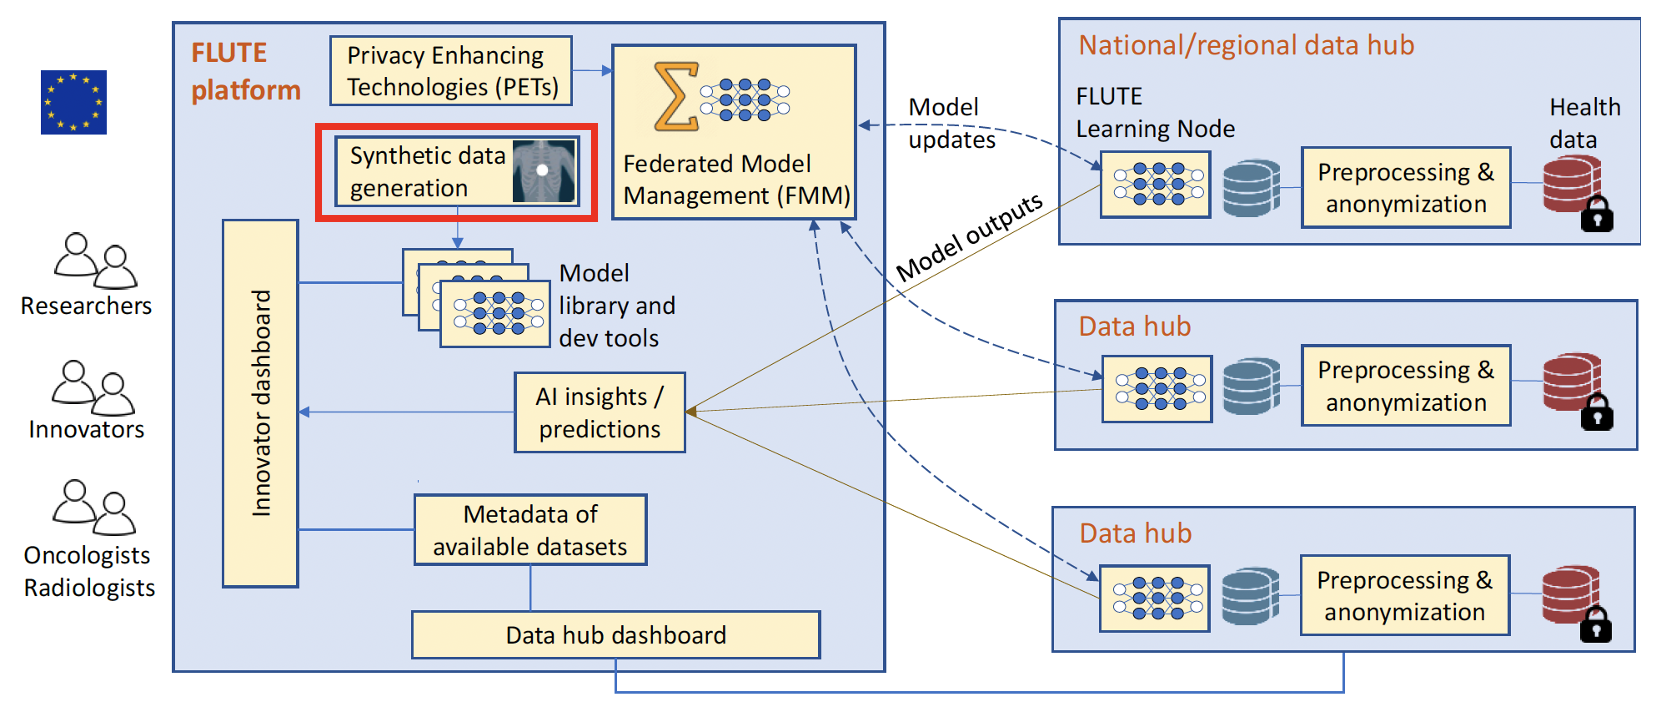
\includegraphics[width=0.9\textwidth]{pics/methodology1.png}
    \caption{Synthetic data generation module (framed in red) into the FLUTE value chain and high level architecture}
    \label{fig:methodology1}
\end{figure}


\begin{figure}[htb]
    \centering
    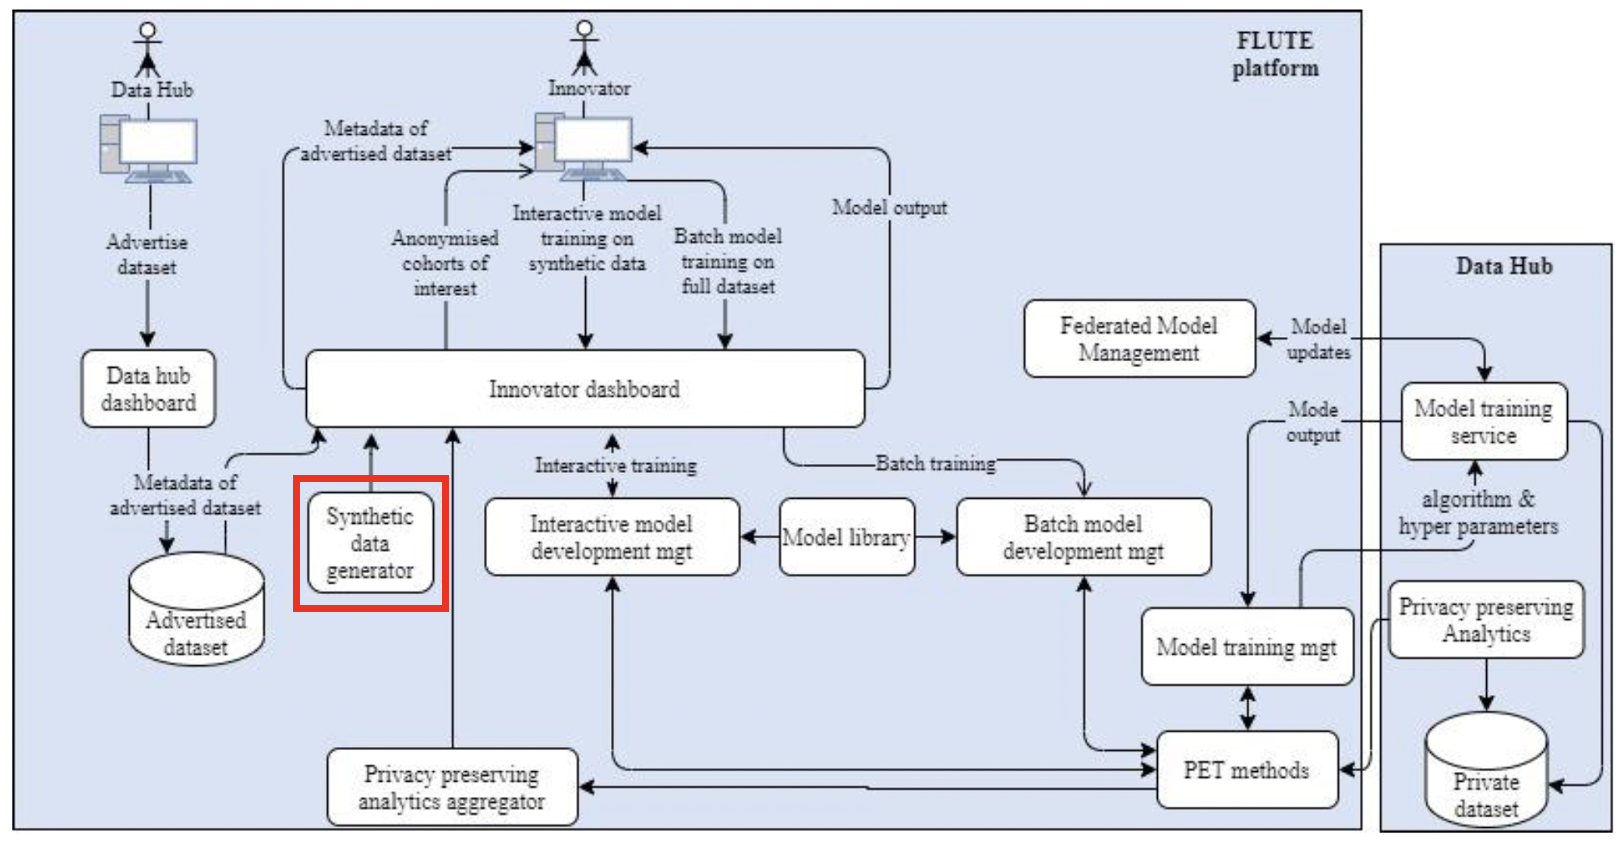
\includegraphics[width=0.9\textwidth]{pics/methodology2.png}
    \caption{Synthetic data generation module (framed in red) into the reference implementation architecture of FLUTE platform}
    \label{fig:methodology2}
\end{figure}

\begin{figure}[htb]
    \centering
    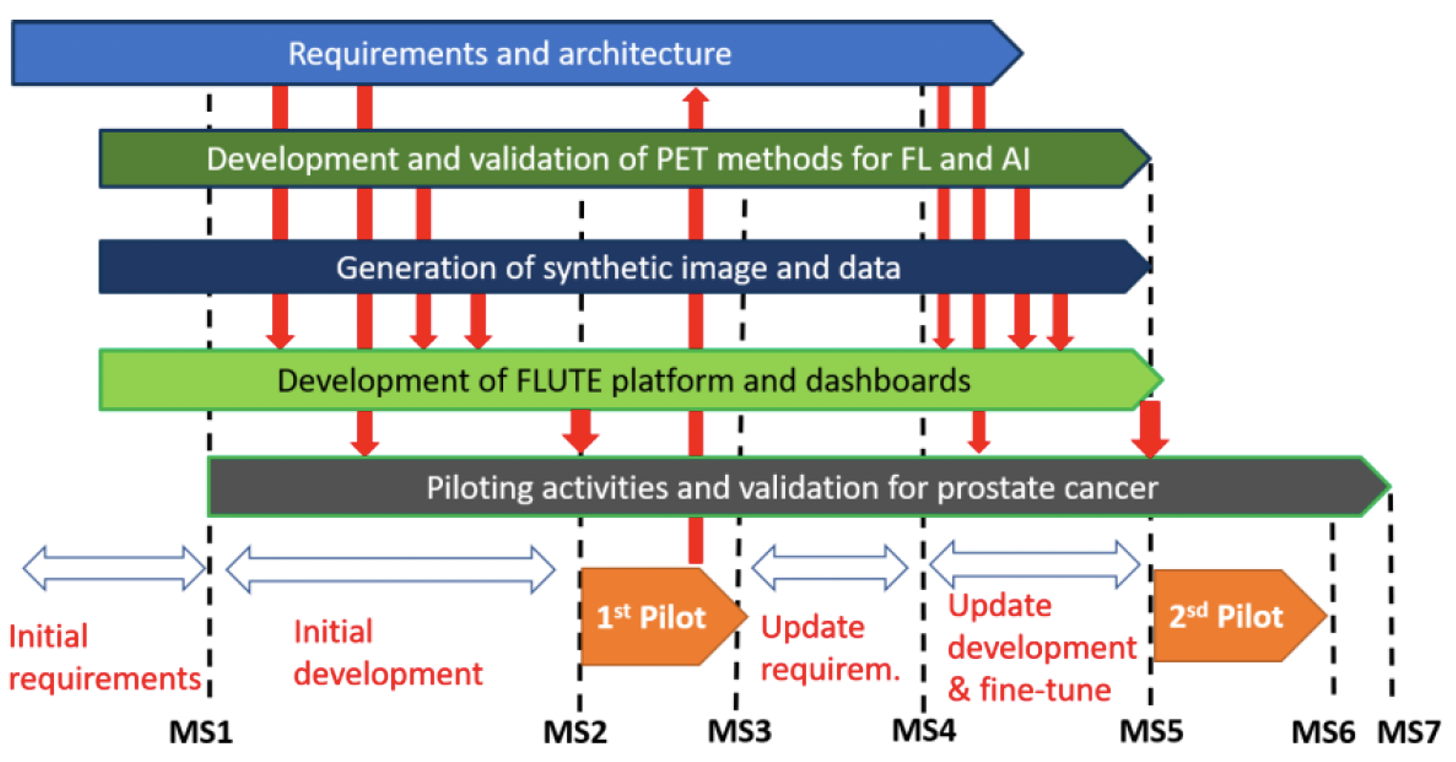
\includegraphics[width=0.75\textwidth]{pics/methodology3.png}
    \caption{Project flow and 2-stage clinical validation}
    \label{fig:methodology3}
\end{figure}

\begin{figure}[htb]
    \centering
    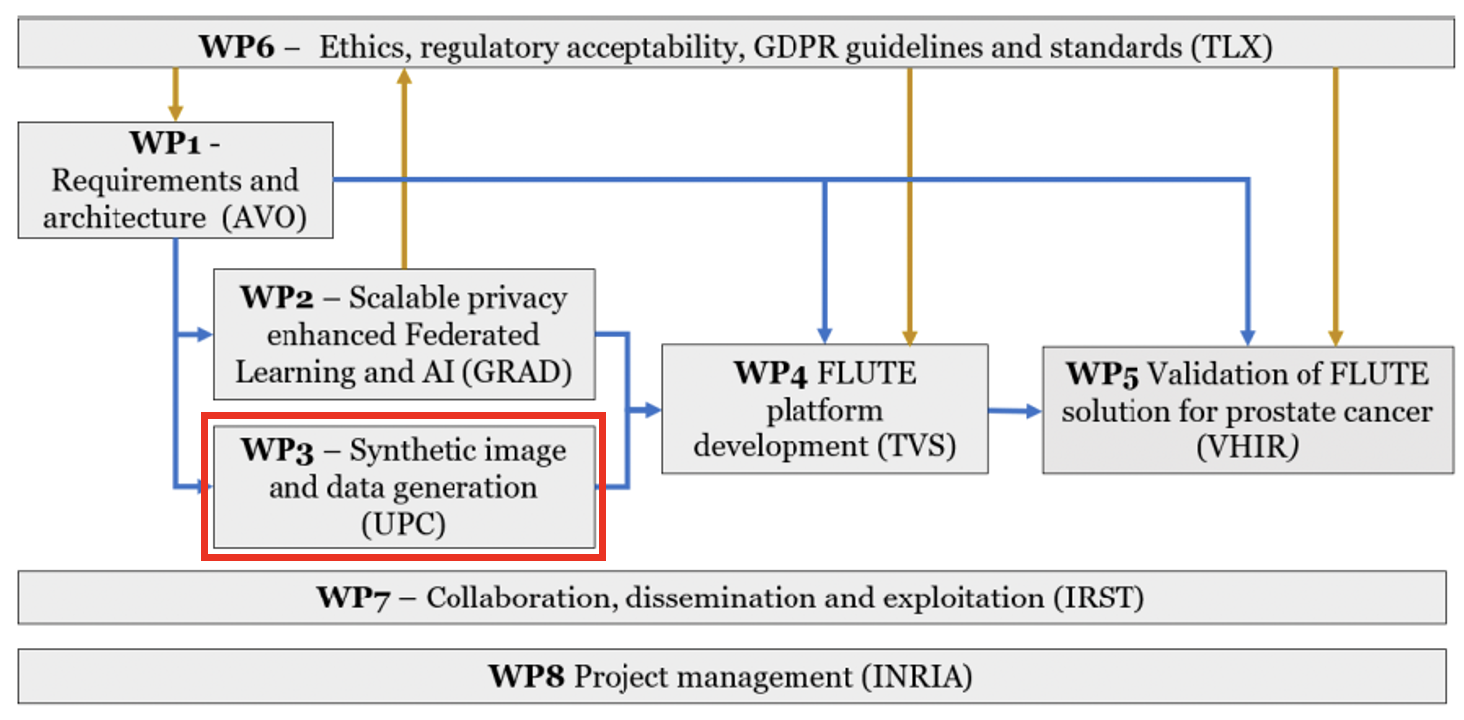
\includegraphics[width=0.75\textwidth]{pics/methodology4.png}
    \caption{Synthetic image and data generation work package (framed in red) into the FLUTE work plan overview}
    \label{fig:methodology4}
\end{figure}


\section{State of the Art}

This section is devoted to the state of the art about novel methods of synthetic healthcare data generation. 

As it was written in the project application, health data hubs may contain data in different formats. The multicategory logical, date, ordinal and continuous data from the hospitals are typically in the form of EHRs, while oncology data lakes provide biopsy and biparameteric (bp) and multiparametric (mp) MRI images and measured variables of the tumors, such as size, position and volume. The EHRs and parameters extracted from MRI are usually
converted into 2-D objects that can be processed by Generative Adversarial Networks (GANs) to generate synthetic
data: specifically for cancer patients~\cite{GonzalezAbriletal2021}, or medGAN~\cite{Choietal2017} and MC-medGAN~\cite{Caminoetal2018} for EHRs-based secure federated AI model development. In FLUTE, these will be extended to generate novel multi-modal information. Moreover, novel
approaches using auto-encoder structures as well as GPT / BERT architectures, that currently use 1-D data, will be
explored by constructing multi-modal datasets in the form of 1-D objects~\cite{Chenetal2020}. For bpMRI and mpMRI, the existing
models are limited to the generation of 2D slices or small patches due to memory constraints~\cite{Daretal2019}. In FLUTE, new
models based on GANs and Autoencoders will be developed to generate full 3D volumes. Two approaches will be
considered: (a) based on the synthesis of a single parametric MRI and image-to-image translation, generate the other
MRI modalities; (2) generate all modalities in a single stage while ensuring the consistency of the parametric information. Novel uses of synthetic data in FL will be applied based on recent work~\cite{Emametal2020} with insertion in FL considered
to be a form of data augmentation for training local models on local and synthetic global data.

\subsection{Generative AI market}
Synthetic data generation, generative systems in general, are engaging the most powerful AI revolution since AI was coined on discriminative models. This is true, not only from the scientific side, but the Industry and Society. For instance, Mistral AI (https://mistral.ai/) a company only four weeks old promising to develop ``the best (open-source) generative AI models'' is valued at \$260 million. France’s Mistral AI blows in with a \$113M seed round to take on OpenAI, the ChatGPT's company~\cite{BraAbb2023}.

Gartner was forecasting in 2021 how synthetic data will completely overshadow real data in AI models by 2030~\cite{Toews2023} (see \figurename~\ref{fig:gartner}).

\begin{figure}[htb]
    \centering
    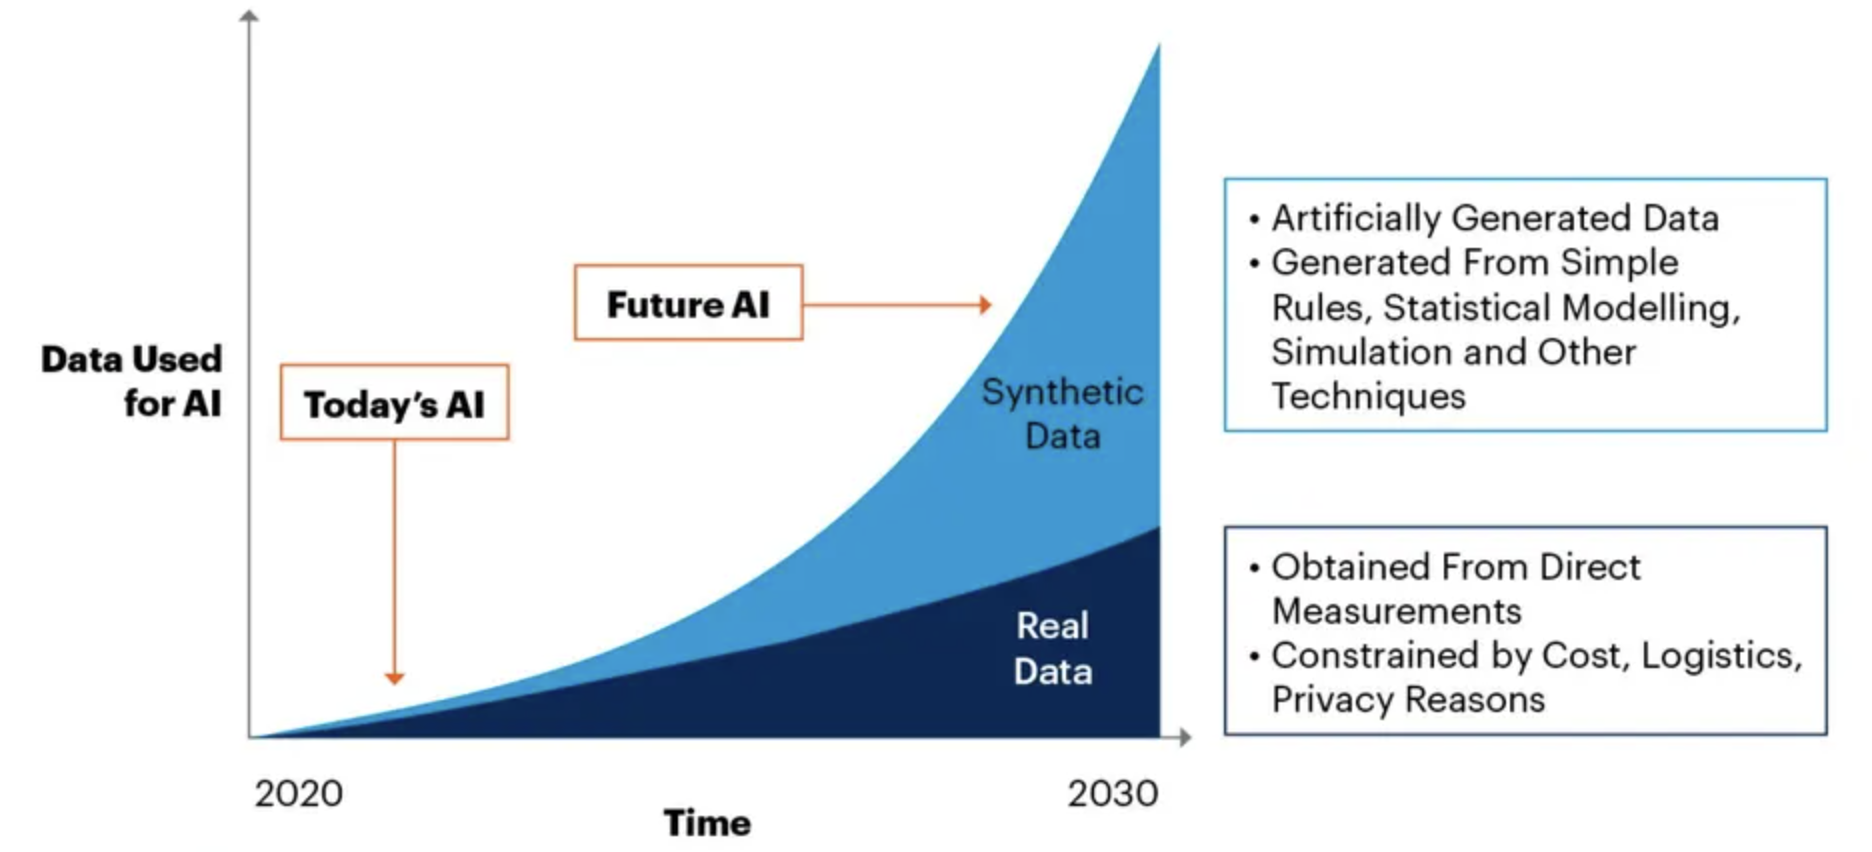
\includegraphics[width=0.75\textwidth]{pics/gartner.png}
    \caption{Synthetic image and data generation work package (framed in red) into the FLUTE work plan overview}
    \label{fig:gartner}
\end{figure}

\newpage

\bibliographystyle{plain}
\bibliography{biblio}

\end{document}
